\chapter{Linear Classification at the Top}\label{chap: linear}

\begin{mini}{\bm{w}}{
  \lambda_1 \cdot \fp(\bm{s}, t) + \lambda_2 \cdot \fn(\bm{s}, t)
}{\label{eq: aatp linear}}{}
  \addConstraint{s_i}{= \bm{w}^{\top}\bm{x}_i , \quad}{i = 1, 2, \ldots, n}
  \addConstraint{t}{= G(\Brac[c]{\bm{s}_i; y_i}_{i \in \I}),}
\end{mini}

% For samples~$\bm{x}$, we consider the linear classifier~$f(\bm{w}) = \bm{w}^\top \bm{x} - t$, where~$\bm{w}$ is the normal vector to the separating hyperplane and~$t$ is a threshold. The most well-known example is the support vector machines, where~$t$ is an optimization variable. In many cases the threshold~$t$ is computed from the scores~$s = \bm{w}^\top \bm{x}$. For example, \TopPush from~\cite{li2014top} sets the threshold~$t$ to the largest score~$s^-$ corresponding to negative samples and~\cite{grill2016learning} sets it to the quantile of all scores.

\section{Theoretical Analysis of the Framework}\label{sec:theory}

In this section, we provide a theoretical analysis of the unified framework from Chapter~\ref{chap: framework} with linear classifier. We consider purely the problem \textit{formulations} and not individual \textit{algorithms} which specify how to solve these formulations. We focus mainly on the following desirable properties:
\begin{itemize}
  \item \textit{Convexity} implies a guaranteed convergence for many optimization algorithms or their better convergence rates~\cite{boyd2004convex}.
  \item \textit{Differentiability} increases the speed of convergence.
  \item \textit{Stability} is a general term, by which we mean that the global minimum is not at~$\bm{w} = \bm{0}$. This actually happens for many formulations from Chapter~\ref{chap: framework} and results in the situation where the separating hyperplane is degenerate and does not actually exist.
\end{itemize}
For a nicer flow of text, we show the results only for formulations from Section~\ref{sec: aatp}. The results for methods from Section~\ref{sec: Neyman-Pearson} are identical. For the same reason, we postpone the proofs to Appendix~\ref{app: proofs primal}.

\subsection{Convexity}\label{sec:convexity}

Convexity is one of the most important properties in numerical optimization. It ensures that the optimization problem has neither stationary points nor local minima. All points of interest are global minima. Moreover, it allows for faster convergence rates. We present the following two results.

\begin{restatable}{proposition}{propconvex}\label{prop:convex}
  Thresholds~$t_2$ and~$t_3$ are convex functions of the weights~$\bm{w}$. The threshold function~$t_1$ is non-convex.
\end{restatable}

\begin{restatable}{theorem}{thmconvex}\label{thm:convex}
  If the threshold~$t$ is a convex function of the weights~$\bm{w}$, then function~$f(\bm{w}) = \fns(\bm{w}, t(\bm{w}))$ is convex.
\end{restatable}

While the proof of Theorem~\ref{thm:convex} is simple, it points to the necessity of considering only false-negatives in the objective of the problems in Chapter~\ref{chap: framework}. In such a case, \TopPush, \TopPushK, \TopMeanK, \tauFPL, \PatMat and \PatMatNP are convex problems. At the same time, \Grill and \GrillNP are not convex problems.

\subsection{Differentiability}

Similarly to convexity, differentiability allows for faster convergence rate and in some algorithms, better termination criteria. The next theorem shows which formulations are differentiable.

\begin{restatable}{theorem}{derivative}\label{thm:derivative}
  If the surrogate function~$l$ is differentiable, then threshold~$t_3$ is a differentiable function of the weights~$\bm{w}$ and its derivative equals to
  \begin{equation*}
    \nabla t_3(\bm{w}) = \frac{\sum_{\bm{x} \in \Xc} l'(\beta(\bm{w}^\top \bm{x} - t_3(\bm{w})))\bm{x}}{\sum_{\bm{x} \in \Xc}l'(\beta(\bm{w}^\top \bm{x} - t_3(\bm{w})))}.
  \end{equation*}
  The threshold functions~$t_1$ and~$t_2$ are non-differentiable.
\end{restatable}

\noindent This theorem shows that the objective functions of \PatMat and \PatMatNP are differentiable. This allows us to prove the convergence of the stochastic gradient descent for these two formulations in Section~\ref{sec:convergence}.

\subsection{Stability}\label{sec: stability}

We first provide a simple example and show that many formulations from the previous section are degenerate for it. Then we analyze general conditions under which this degenerate behaviour happens.

\subsubsection{Example of a Degenerate Behavior}\label{sec:example}

We consider~$n$ negative samples uniformly distributed in~$[-1,0]\times[-1,1]$,~$n$ positive samples uniformly distributed in~$[0,1]\times[-1,1]$ and one negative sample at~$(2,0)$, see Figure~\ref{fig:example} (left). We consider the hinge loss and no regularization. If~$n$ is large, the point at~$(2,0)$ is an outlier and the dataset is separable and the separating hyperplane has the normal vector~$\bm{w}=(1,0)$. 

\begin{figure}[!ht]
  \centering
  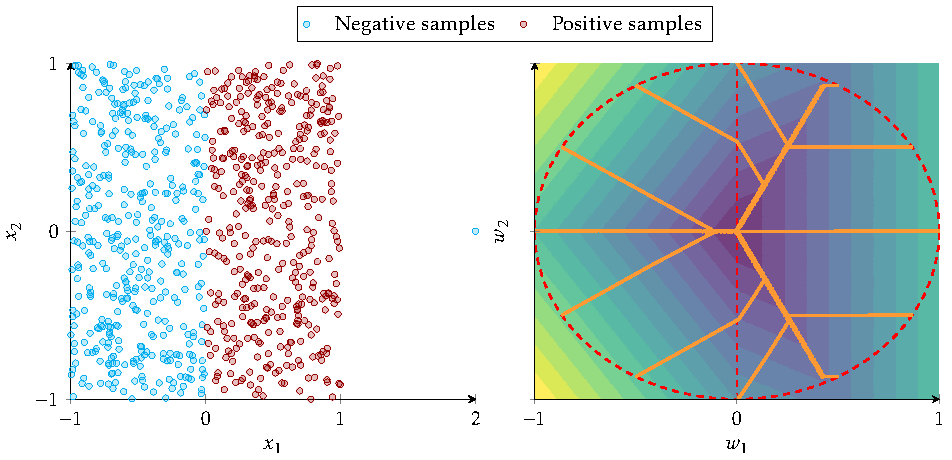
\includegraphics[width=0.7\linewidth]{images/toppush_convergence.pdf}
  \caption{Left: distribution of positive (empty circle) and negative samples (full circles) for the example from Section~\ref{sec:example}. Right: contour plot for \TopPush and its convergence to the zero vector from~$12$ initial points.}
  \label{fig:example}
\end{figure}

Table~\ref{tab:example} shows the threshold~$t$ and the objective value~$f$ for two points~$\bm{w}_1=(0,0)$ and~$\bm{w}_2=(1,0)$. These two points are both important:~$\bm{w}_1$ does not generate any separating hyperplane, while~$\bm{w}_2$ generates the optimal separating hyperplane. We show the precise computation in Appendix~\ref{app:example}. Since the dataset is perfectly separable by~$\bm{w}_2$, we expect that~$\bm{w}_2$ provides a lower objective than~$\bm{w}_1$. By shading the better objective in Table~\ref{tab:example} by grey, we see that this did not happen for \TopPush and \TopMeanK.

\begin{table}[!ht]
  \centering
  \begin{tabular}{@{}l ccccc@{}}\toprule
    & & \multicolumn{2}{c}{$\bm{w}_1=(0,0)$} & \multicolumn{2}{c}{$\bm{w}_2=(1,0)$} \\ \cmidrule(lr){3-4} \cmidrule(lr){5-6}
    Name & Label & $t$& $f$ & $t$ & $f$ \\
    \midrule
    \TopPush & \eqref{eq: toppush surrogate} & $0$ & \cellcolor{gray!40}$1$ & $2$ & $2.5$ \\
    \TopPushK & \eqref{eq: toppushK surrogate} & $0$ & $1$ & $\frac2k$ & \cellcolor{gray!40}$0.5+\frac2k$ \\
    \Grill & \eqref{eq: grill} & $0$ & $2$ & $1-2\tau$ & \cellcolor{gray!40}$1.5+2\tau(1-\tau)$ \\
    \TopMeanK & \eqref{eq: topmeank} & $0$ & \cellcolor{gray!40}$1$ & $1-\tau$ & $1.5-\tau$ \\
    \PatMat & \eqref{eq: patmat}  & $\frac{1}{\beta}(1-\tau)$ & $1+\frac{1}{\beta}(1-\tau)$ & $\frac{1}{\beta}(1-\tau)$ & \cellcolor{gray!40}$0.5+\frac{1}{\beta}(1-\tau)$ \\
    \bottomrule
  \end{tabular}
  \caption{Comparison of formulations on the very simple problem from Section~\ref{sec:example}. Two formulations have the global minimum (denoted by grey color) at~$\bm{w}_1=(0,0)$ which does not generate any separating hyperplane. The optimal separating hyperplane is generated by~$\bm{w}_2=(1,0)$.}
  \label{tab:example}
\end{table}

It can be shown that~$\bm{w}_1=(0,0)$ is even the global minimum for \TopPush and \TopMeanK. This raises the question of whether some tricks, such as early stopping or excluding a small ball around zero, cannot overcome this difficulty. The answer is negative as shown in Figure~\ref{fig:example} (right). Here, we run \TopPush from several starting points, and it always converges to zero from one of the three possible directions; all of them far from the normal vector to the separating hyperplane.

\subsubsection{Stability and Global minimum at zero}\label{sec:w_zero}

The convexity derived in the previous section guarantees that there are no local minima. However, as we showed in the example above, the global minimum may be at~$\bm{w} = \bm{0}$. This is highly undesirable since~$\bm{w}$ is the normal vector to the separating hyperplane and the zero vector provides no information. In this section, we analyze when this situation happens. The first result states that if the threshold~$t(\bm{w})$ is above a certain value, then zero has a better objective that~$\bm{w}$. If this happens for all~$\bm{w}$, then zero is the global minimum.

\begin{restatable}{theorem}{larget}\label{thm:large_t}
  Consider any of these formulations: \TopPush, \TopPushK, \TopMeanK or \tauFPL. Fix any~$\bm{w}$ and denote the corresponding threshold~$t(\bm{w})$. If we have
  \begin{equation}\label{eq:w_zero_nn}
    t(\bm{w})\ge \frac{1}{n^+} \sum_{\bm{x}^+ \in \Xc^+} \bm{w}^\top \bm{x}^+,
  \end{equation}
  then~$f(\bm{0})\le f(\bm{w})$. Specifically, denote the scores~$s^+=\bm{w}^\top \bm{x}^+$ for~$\bm{x}^+\in \Xc^+$ and~$s^-=\bm{w}^\top \bm{x}^-$ for~$\bm{x}^-\in \Xc^-$ and the ordered variants with decreasing components of~$\bm{s}^-$ by~$\bm{s}_{[\cdot]}^-$. Then
  \begin{equation}\label{eq:w_zero}
    \begin{aligned}
    s_{[1]}^- \ge \frac{1}{n^+} \sum_{i=1}^{n^+} s_{i}^+
    & \implies f(\bm{0}) \le f(\bm{w}) \text{ for } \TopPush, \\
    \frac{1}{k}\sum_{i=1}^k s_{[i]}^- \ge \frac{1}{n^+} \sum_{i=1}^{n^+} s_{i}^+
    & \implies f(\bm{0})\le f(\bm{w}) \text{ for } \TopPushK, \\
    \frac{1}{n^-\tau} \sum_{i=1}^{n^-\tau} s_{[i]}^- \ge \frac{1}{n^+}\sum_{i=1}^{n^+} s_{i}^+
    & \implies f(\bm{0}) \le f(\bm{w}) \text{ for } \tauFPL. \\
    \end{aligned}
  \end{equation}
\end{restatable}

We can use this result immediately to deduce that some formulations have the global minimum at~$\bm{w} = \bm{0}$. More specifically, \TopPush fails if there are outliers, and \TopMeanK fails whenever there are many positive samples.

\begin{corollary}\label{cor:toppush}
  Consider the \TopPush formulation. If the positive samples lie in the convex hull of negative samples, then~$\bm{w}=\bm{0}$ is the global minimum.
\end{corollary}

\begin{corollary}\label{cor:topmean}
  Consider the \TopMeanK formulation. If~$n^+\ge n\tau$, then~$\bm{w}=\bm{0}$ is the global minimum.
\end{corollary}

The proof of Theorem~\ref{thm:large_t} employs the fact that all formulations in the theorem statement have only false-negatives in the objective. If~$\bm{w}_0=\bm{0}$, then~$\bm{w}_0^\top \bm{x}=0$ for all samples~$\bm{x}$, the threshold equals to~$t=0$ and the objective equals to one. If the threshold is large for~$\bm{w}$, many positives are below the threshold, and the false-negatives have the average surrogate value larger than one. In such a case,~$\bm{w}_0=\bm{0}$ becomes the global minimum. There are two fixes to this situation:
\begin{itemize}
  \item Include false-positives to the objective. This approach is taken by \Grill and \GrillNP and necessarily results in the loss of convexity.  \item Move the threshold away from zero even when all scores~$\bm{w}^\top \bm{x}$ are zero. This approach is taken by our formulations \PatMat and \PatMatNP and keeps convexity.
\end{itemize}
The next theorem shows the advantage of the second approach.

\begin{restatable}{theorem}{patmatzero}\label{thm:patmat_zero}
  Consider the \PatMat or \PatMatNP formulation with the hinge surrogate and no regularization. Assume that for some~$\bm{w}$ we have
  \begin{equation}\label{eq:patmat_zero}
    \frac{1}{n^+}\sum_{\bm{x}^+ \in \Xc^+}\bm{w}^\top \bm{x}^+ > \frac{1}{n^-}\sum_{\bm{x}^- \in \Xc^-}\bm{w}^\top \bm{x}^-.
  \end{equation}
  Then there is a scaling parameter~$\beta_0$ from \eqref{eq: aatp quantile surrogate} such that~$f(\bm{w})<f(\bm{0})$ for all~$\beta\in(0,\beta_0)$.
\end{restatable}

These theorem shed some light on the behaviour of the formulations. Theorem~\ref{thm:large_t} states that the stability of \tauFPL requires
\begin{equation}\label{eq:stability1}
  \frac{1}{n^-\tau}\sum_{i=1}^{n^-\tau}s_{[i]}^- < \frac{1}{n^+}\sum_{i=1}^{n^+} s_{i}^+,
\end{equation}
while Theorem~\ref{thm:patmat_zero} states that the stability of \PatMatNP is ensured by
\begin{equation}\label{eq:stability2}
  \frac{1}{n^-}\sum_{i=1}^{n^-}s_{[i]}^- < \frac{1}{n^+}\sum_{i=1}^{n^+} s_{i}^+.
\end{equation}
The right-hand sides of \eqref{eq:stability1} and \eqref{eq:stability2} are the same, while the left-hand side of \eqref{eq:stability2} is always smaller than the left-hand side of \eqref{eq:stability1}. This implies that if \tauFPL is stable, then \PatMatNP is stable as well.

At the same time, there may be a huge difference in the stability of both formulations. Since the scores of positive samples should be above the scores of negative samples, the scores~$s$ may be interpreted as performance. Then formula \eqref{eq:stability1} states that if the mean performance of a \emph{small number of the best} negative samples is larger than the average performance of \emph{all} positive samples, then \tauFPL fails. On the other hand, formula \eqref{eq:stability2} states that if the average performance of \emph{all} positive samples is better than the average performance of \emph{all} negative samples, then \PatMatNP is stable. The former may well happen as accuracy at the top is interested in a good performance of only a small number of positive samples.

\subsection{Method comparison}

We provide a summary of the obtained results in Table~\ref{tab:methods}. There we give basic characterizations of the formulations such as their definition label, their source, the hyperparameters, whether the formulation is differentiable and convex, and whether it has stability problems with~$\bm{w}=\bm{0}$ being the global minimum. 

\begin{table}[!ht]
  \centering
  \begin{tabular}{ll ccccc}\toprule
    Name & Source & Definition & Hyperpars & Convex & Differentiable & Stable \\
    \midrule
    \TopPush &~\cite{li2014top} & \eqref{eq: toppush surrogate}&~$\lambda$ & \yesmark & \nomark & \nomark\\
    \TopPushK & ours & \eqref{eq: toppushK surrogate} &~$\lambda$,~$k$ & \yesmark & \nomark & \nomark\\ 
    \Grill &~\cite{grill2016learning} & \eqref{eq: grill}  &~$\lambda$ & \nomark & \nomark & \yesmark\\
    \PatMat & ours & \eqref{eq: patmat} &~$\beta$,~$\lambda$ & \yesmark & \yesmark & \yesmark\\ 
    \TopMeanK & - & \eqref{eq: topmeank} &~$\lambda$ & \yesmark & \nomark & \nomark\\ 
    \GrillNP & - & \eqref{eq:problem_grill_np} &~$\lambda$ & \nomark & \nomark & \yesmark\\
    \PatMatNP & ours & \eqref{eq:problem_patmat_np} &~$\beta$,~$\lambda$ & \yesmark & \yesmark & \yesmark\\
    \tauFPL &~\cite{zhang2018tau} & \eqref{eq:problem_topmeank_np} &~$\lambda$ & \yesmark & \nomark & \nomark\\
    \bottomrule
  \end{tabular}
  \caption{Summary of the formulations from Chapter~\ref{chap: framework}. The table shows their definition label, the source or the source they are based on, the hyperparameters, whether the formulation is differentiable, convex and stable (in the sense of having problems with~$\bm{w}=\bm{0}$).}
  \label{tab:methods}
\end{table}

A similar comparison is performed in Figure~\ref{fig:thresholds}. Methods in green and grey are convex, while formulations in white are non-convex. Based on Theorem~\ref{thm:large_t}, four formulations in grey are vulnerable to have the global minimum at~$\bm{w}=0$. This theorem states that the higher the threshold, the more vulnerable the formulation is. The full arrows depict this dependence. If it points from one formulation to another, the latter one has a smaller threshold and thus is less vulnerable to this undesired global minima. The dotted arrows indicate that this holds usually but not always, the precise formulation is provided in Appendix~\ref{app:relations}. This complies with Corollaries~\ref{cor:toppush} and~\ref{cor:topmean} which state that \TopPush and \TopMeanK are most vulnerable. At the same time, it says that \tauFPL is the best one from the grey-coloured formulations. Finally, even though \PatMatNP has a worse approximation of the true threshold than \tauFPL due to Theorem~\ref{thm:large_t}, it is more stable due to the discussion after Theorem~\ref{thm:patmat_zero}.

\begin{figure}[!ht]
  \centering
  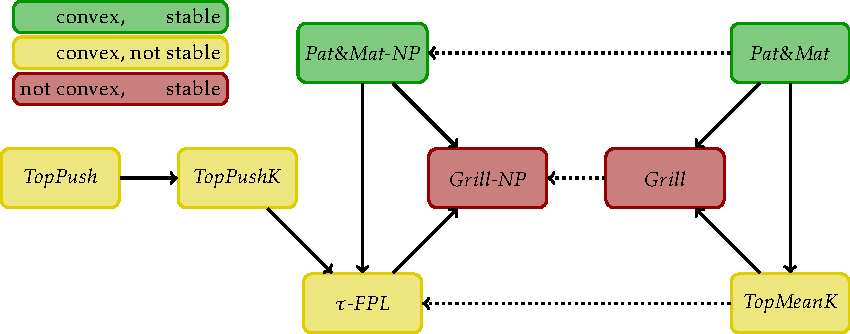
\includegraphics[width = \linewidth]{images/methods_relation.pdf}
  \caption{Summary of the formulations from Chapter~\ref{chap: framework}. Methods in green and grey are convex, while formulations in white are non-convex. Methods in grey are vulnerable to have the global minimum at~$\bm{w}=0$. Full (dotted) arrow pointing from one formulation to another show that the latter formulation has always (usually) smaller threshold.}
  \label{fig:thresholds}
\end{figure}

\section{Convergence of stochastic gradient descent}\label{sec:convergence}

The previous section analyzed the formulations from Chapter~\ref{chap: framework} but did not consider any optimization algorithms. In this section, we show a basic version of the stochastic gradient descent and then show its convergent version. Since due to considering the threshold, gradient computed on a minibatch is a biased estimate of the true gradient, we need to use variance reduction techniques, and the proof is rather complex.

\subsection{Stochastic gradient descent: Basic}

Many optimization algorithms for solving the formulations from Chapter~\ref{chap: framework} use primal-dual or purely dual formulations.~\cite{eban2017scalable} introduced dual variables and used alternating optimization to the resulting min-max problem. ~\cite{li2014top} and~\cite{zhang2018tau} dualized the problem and solved it with the steepest gradient ascent.~\cite{macha2020nonlinear} followed the same path but added kernels to handle non-linearity. We follow the ideas of~\cite{mackey2018constrained} and~\cite{adam2019machine} and solve the problems directly in their primal formulations. Therefore, even though we use the same formulation for \TopPush as~\cite{li2014top} or for \tauFPL as~\cite{zhang2018tau}, our solution process is different. However, due to convexity, both algorithms should converge to the same point.

The decision variables in \eqref{eq: aatp surrogate} are the normal vector of the separating hyperplane~$\bm{w}$ and the threshold~$t$. To apply an efficient optimization method, we need to compute gradients. The simplest idea~\cite{grill2016learning} is to compute the gradient only with respect to~$\bm{w}$ and then recompute~$t$. A more sophisticated way is based on the chain rule. For each~$\bm{w}$, the threshold~$t$ can be computed uniquely. We stress this dependence by writing~$t(\bm{w})$ instead of~$t$. By doing so, we effectively remove the threshold~$t$ from the decision variables and~$\bm{w}$ remains the only decision variable. Note that the convexity is preserved. Then we can compute the derivative via the chain rule
\begin{equation}\label{eq:derivatives}
  \begin{aligned}
  f(\bm{w}) & = \frac{1}{n^+}\sum_{\bm{x} \in \Xc^+} l(t(\bm{w}) - \bm{w}^\top \bm{x}) + \frac{\lambda}{2}\norm{\bm{w}}^2, \\
  \nabla f(\bm{w}) & = \frac{1}{n^+}\sum_{\bm{x} \in \Xc^+} l'(t(\bm{w}) - \bm{w}^\top \bm{x})(\nabla t(\bm{w}) - \bm{x}) + \lambda \bm{w}.
  \end{aligned}
\end{equation}
The only remaining part is the computation of~$\nabla t(\bm{w})$. It is simple for~$\nabla t_1(\bm{w})$ and~$\nabla t_2(\bm{w})$ and Theorem~\ref{thm:derivative} shows the computation for~$\nabla t_3(\bm{w})$. Appendix~\ref{app:threshold} provides an efficient computation method for~$t_3(\bm{w})$.

Having derivative \eqref{eq:derivatives}, deriving the stochastic gradient is simple. It partitions the dataset into minibatches and provides an update of the weights~$\bm{w}$ based only on a minibatch, namely by replacing the mean over the whole dataset in \eqref{eq:derivatives} by a mean over the minibatch.

\subsection{Stochastic gradient descent: Convergent for \PatMat and \PatMatNP}

For the convergence proof, we need differentiability which is due to Theorem~\ref{thm:derivative} possessed only by \PatMat and \PatMatNP. Therefore, we consider only these two formulations and for simplicity, show it only for \PatMat. We apply a variance reduction technique based on delayed values similar to SAG~\cite{schmidt2017minimizing}. 

At iteration~$k$ we have the decision variable~$\bm{w}^k$ and the active minibatch~$I^k$. First, we update the score vector~$\bm{s}^k$ only on the active minibatch by setting
\begin{equation}\label{eq:defin_z}
  s_i^k = \begin{cases} \bm{x}_i^\top \bm{w}^k &\text{for all }i\in I^k,\\ s_i^{k-1} &\text{for all }i\notin I^k.\end{cases} 
\end{equation}
We keep scores from previous minibatches intact. We use Appendix~\ref{app:threshold} to compute the surrogate quantile~$t^k$ as the unique solution of
\begin{equation}\label{eq:update_t}
  \sum_{i \in X}l(\beta(s_i^k - t^k)) = n\tau.
\end{equation}
This is an approximation of the surrogate quantile~$t(\bm{w}^k)$ from \eqref{eq: aatp quantile surrogate}. The only difference from the true value~$t(\bm{w}^k)$ is that we use delayed scores. Then we introduce artificial variable
\begin{equation}\label{eq:update_a}
  \begin{aligned}
    \bm{a}^k &= \sum_{i\in I^k}l'(\beta(s_i^k - t^k))\bm{x}_i.
  \end{aligned}
\end{equation}
Finally, we approximate the derivative~$\nabla f(\bm{w}^k)$ from \eqref{eq:derivatives} by
\begin{equation}\label{eq:update_g}
  g(\bm{w}^k) = \frac{1}{n^k_+}\sum_{i\in I^k_+}l'(t^k - s_i^k)(\nabla t^k - \bm{x}_i),
\end{equation}
where~$\nabla t^k$ is an approximation of~$\nabla t(\bm{w}^k)$ from Theorem~\ref{thm:derivative} defined by
\begin{equation}\label{eq:update_nablat}
  \nabla t^k = \frac{\bm{a}^k + \bm{a}^{k-1} + \dots + \bm{a}^{k - m + 1}}{\sum_{i \in X} l'(\beta(s_i^k - t^k))}.
\end{equation}
A perhaps more straightforward possibility would be to consider only~$\bm{a}^k$ in the numerator of \eqref{eq:update_nablat}. However, choice \eqref{eq:update_nablat} enables us to prove the convergence and it adds stability to the algorithm for small minibatches.

The whole procedure does not perform any vector operations outside of the current minibatch~$I^k$. We summarize it in Algorithm~\ref{alg:sgd}. Note that a proper initialization for the first~$m$ iterations is needed. We finish the theoretical part by the convergence proof.

\begin{algorithm}[!ht]
  \begin{algorithmic}[1]
    \Require Dataset~$X$, Minibatches~$I^1,\dots,I^m$, Stepsize~$\alpha^k$
    \State Initialize weights~$\bm{w}^0$
    \For{$k = 0,1,\dots$}
    \State Select a minibatch~$I^k$
    \State Compute~$s_i^k$ for all~$i\in I^k$ according to \eqref{eq:defin_z}
    \State Compute~$t^k$ according to \eqref{eq:update_t}
    \State Compute~$\bm{a}^k$ according to \eqref{eq:update_a}
    \State Compute~$\nabla t^k$ according to \eqref{eq:update_nablat}
    \State Compute~$g(\bm{w}^k)$ according to \eqref{eq:update_g}
    \State Set~$\bm{w}^{k+1}\gets \bm{w}^k - \alpha^k g(\bm{w}^k)$
    \EndFor
  \end{algorithmic}
  \caption{Stochastic gradient descent for maximizing accuracy at the top}
  \label{alg:sgd}
\end{algorithm}

\begin{restatable}{theorem}{sgd}\label{thm:sgd}
  Consider the \PatMat or \PatMatNP formulation, stepsizes~$\alpha^k = \frac{\alpha^0}{k+1}$ and piecewise disjoint minibatches~$I^1,\dots,I^m$ which cycle periodically~$I^{k+m}=I^k$. If~$l$ is the smoothened (Huberized) hinge function, then Algorithm~\ref{alg:sgd} converges to the global minimum of \eqref{eq: patmat}.  
\end{restatable}

\section{Numerical experiments}\label{sec:num1}

In this section, we present numerical results.

\subsection{Implementational details and Hyperparameter choice}

We recall that all methods fall into the framework of either \eqref{eq: aatp counts} or \eqref{eq: aatp surrogate}. Since the threshold~$t$ depends on the weights~$\bm{w}$, we can consider the decision variable to be only~$\bm{w}$. Then to apply a method, we implemented the following iterative procedure. At iteration~$j$, we have the weights~$\bm{w}^j$ to which we compute the threshold~$t^j=t(\bm{w}^j)$. Then according to \eqref{eq:derivatives}, we compute the gradient of the objective and apply the ADAM descent scheme~\cite{kingma2014adam}. All methods were run for~$10000$ iterations using the stochastic gradient descent. The minibatch size was~$512$ except for the sigillito1989classification and Spambase datasets where the full gradient was used. All methods used the hinge surrogate \eqref{eq:defin_surrogate}. The initial point is generated randomly.

We run the methods for the following hyperparameters
\begin{equation}\label{eq:beta1}
  \begin{aligned}
    \beta   & \in  \{0.0001,\ 0.001,\ 0.01,\ 0.1,\ 1,\ 10\}, \\
    \lambda & \in \{0,\ 0.00001,\ 0.0001,\ 0.001,\ 0.01,\ 0.1\}, \\
    k       & \in \{1, 3, 5, 10, 15, 20\}.
  \end{aligned}
\end{equation}
For \TopPushK, \PatMat and \PatMatNP we fixed~$\lambda=0.001$ to have six hyperparameters for all methods. For all datasets, we choose the hyperparameter which minimized the criterion on the validation set. The results are computed on the testing set which was not used during training the methods.

\TopPush and \tauFPL were originally implemented in the dual. However, to allow for the same framework and the stochastic gradient descent, we implemented it in the primal. These two approaches are equivalent.

\subsection{Dataset description and Performance criteria}\label{sec:datasets}

For the numerical results, we considered 10 datasets summarized in Table~\ref{tab:counts}. They can be downloaded from the UCI repository. sigillito1989classification~\cite{sigillito1989classification} and Spambase are small, baldi2016parameterized~\cite{baldi2016parameterized} contains a large number of samples while guyon2005result~\cite{guyon2005result} contains a large number of features. We also considered six visual recognition datasets: MNIST, FashionMNIST, CIFAR10, CIFAR20, CIFAR100 and SVHN2. MNIST and FashionMNIST are grayscale datasets of digits and fashion items, respectively. CIFAR100 is a dataset of coloured images of items grouped into 100 classes. CIFAR10 and CIFAR20 merge these classes into 10 and 20 superclasses, respectively. SVHN2 contains coloured images of house numbers. As Table~\ref{tab:counts} shows, these datasets are imbalanced.

Each of the visual recognition datasets was converted into ten binary datasets by considering one of the classes~$\{0,\dots,9\}$ as the positive class and the rest as the negative class. The experiments were repeated ten times for each dataset from different seeds, which influenced the starting point and minibatch creation. We use tpr@fpr as the evaluation criterion. This describes the true-positive rate at a prescribed true-negative rate, usually of~$1\%$ or~$5\%$. For the linear classifier~$\bm{w}^\top \bm{x} - t$, it selects the threshold~$t$ so that the desired true-negative rate is satisfied and then computes the true-positive rate for this threshold.

\begin{table}[!ht]
  \centering
  \begin{tabular}{@{}lllllllll@{}}
    \toprule
    &  & \multicolumn{2}{c}{Training} & \multicolumn{2}{c}{Validation} & \multicolumn{2}{c}{Testing} \\ \cmidrule(lr){3-4} \cmidrule(lr){5-6} \cmidrule(l){7-8} 
    & $m$ & $n$ & $\frac{n^+}{n}$ & $n$ & $\frac{n^+}{n}$ & $n$ & $\frac{n^+}{n}$ \\ \midrule
    Ionosphere
      & $34$
      & $175$ & $36.0\%$ & $88$ & $36.4\%$ & $88$ & $35.2\%$ \\
    Spambase
      & $57$
      & $2300$ & $39.4\%$ & $1150$ & $39.4\%$ & $1151$ & $39.4\%$ \\
    Gisette
      & $5000$
      & $1000$ & $50.0\%$ & $1500$ & $50.0\%$ & $500$ & $50.0\%$ \\
    Hepmass
      & $28$
      & $5250000$ & $50.0\%$ & $1750000$ & $50.0\%$ & $3500000$ & $50.0\%$ \\
    MNIST
      & $28 \times 28 \times 1$
      & $44999$ & $11.2\%$ & $15001$ & $11.2\%$ & $10000$ & $11.4\%$ \\
    FashionMNIST
      & $28 \times 28\times 1$
      & $45000$ & $10.0\%$ & $15000$ & $10.0\%$ & $10000$ & $10.0\%$ \\
    CIFAR10
      & $32\times 32\times 3$
      & $37500$ & $10.0\%$ & $12500$ & $10.0\%$ & $10000$ & $10.0\%$ \\
    CIFAR20
      & $32 \times 32\times 3$
      & $37500$ & $5.0\%$ & $12500$ & $5.0\%$ & $10000$ & $5.0\%$ \\
    CIFAR100
      & $32 \times 32\times 3$
      & $37500$ & $1.0\%$ & $12500$ & $1.0\%$ & $10000$ & $1.0\%$ \\
    SVHN2
      & $32 \times 32\times 3$
      & $54944$ & $18.9\%$ & $18313$ & $18.9\%$ & $26032$ & $19.6\%$ \\
    \bottomrule
  \end{tabular}
  \caption{Structure of the used datasets. The training, validation and testing sets show the number of features~$m$, samples~$n$ and the fraction of positive samples~$\frac{n^+}{n}$.}
  \label{tab:counts}
\end{table}

\subsection{Numerical results}

Figure~\ref{fig:ptau} presents the standard ROC (receiver operating characteristic) curves on selected datasets. Since all methods from this paper are supposed to work at low false-positive rates, the~$x$ axis is logarithmic. Both figures depict averages over ten runs with different seeds. The left column depicts CIFAR100 while the right one Hepmass. These are the two more complicated datasets. We selected four representative methods: \PatMat and \PatMatNP as our methods and \TopPush and \tauFPL as state-of-the-art methods. Even though all methods work well, \PatMatNP seems to outperform the remaining methods on most levels of false-positive rate.

\begin{figure}[!ht]
  \centering
  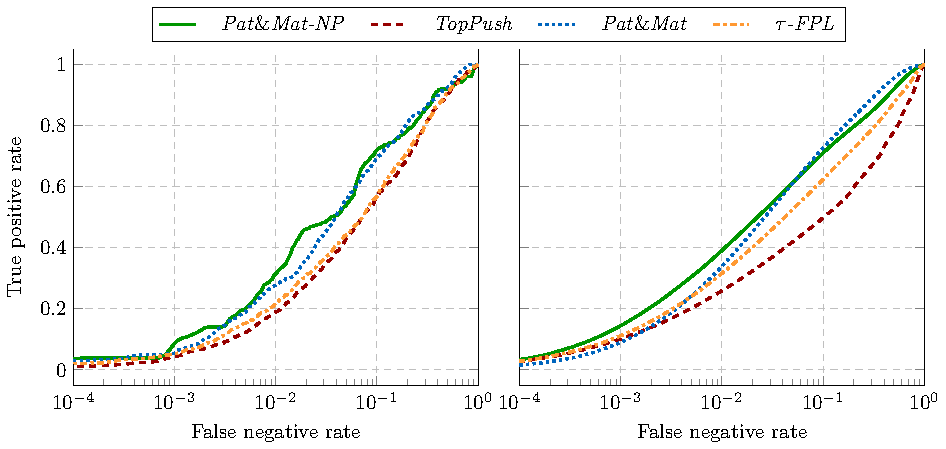
\includegraphics[width = \linewidth]{images/primal_results.pdf}
  \caption{ROC curves (with logarithmic~$x$ axis) on CIFAR100 (left) and Hepmass (right).}
  \label{fig:ptau}
\end{figure}

While Figure~\ref{fig:ptau} gave a glimpse of the behaviour of methods, Figures~\ref{fig:cd1} and~\ref{fig:cd2} provide a statistically more sound comparison. It employs the Nemenyi post hoc test for the Friedman test recommended in~\cite{demvsar2006statistical}. This test compares if the mean ranks of multiple methods are significantly different.

We consider 14 methods (we count different values of~$\tau$ as different methods) as depicted in this table. For each dataset mentioned in Section~\ref{sec:datasets} and each method, we evaluated the fpr@tpr metric and ranked all methods. Rank 1 refers to the best performance for given criteria, while rank 14 is the worst. The~$x$-axis shows the average rank over all datasets. The Nemenyi test computes the critical difference. If two methods are within their critical difference, their performance is not deemed to be significantly different. Black wide horizontal lines group such methods.

\begin{figure}[!ht]
  \centering
  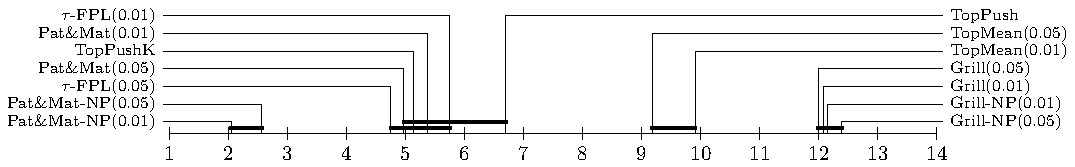
\includegraphics[width = \linewidth]{images/crit_diag_fpr_1.pdf}
  \caption{Critical difference (CD) diagrams (level of importance 0.05) of the Nemenyi post hoc test for the Friedman test. Each diagram shows the mean rank of each method, with rank 1 being the best. Black wide horizontal lines group together methods with the mean ranks that are not significantly different. The critical difference diagrams were computed for mean rank averages over all datasets of the tpr@fpr ($\tau=0.01$) metric.}
  \label{fig:cd1}
\end{figure}

\begin{figure}[!ht]
  \centering
  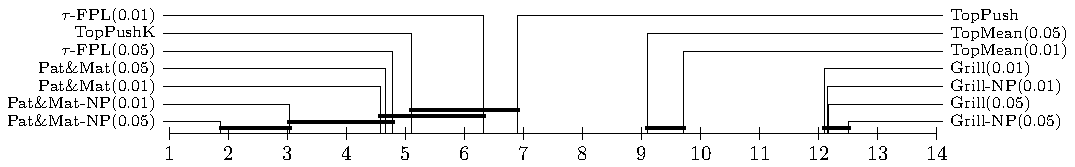
\includegraphics[width = \linewidth]{images/crit_diag_fpr_5.pdf}
  \caption{Critical difference (CD) diagrams (level of importance 0.05) of the Nemenyi post hoc test for the Friedman test. Each diagram shows the mean rank of each method, with rank 1 being the best. Black wide horizontal lines group together methods with the mean ranks that are not significantly different. The critical difference diagrams were computed for mean rank averages over all datasets of the tpr@fpr ($\tau=0.05$) metric.}
  \label{fig:cd2}
\end{figure}

From this figure and table, we make several observations:
\begin{itemize}
  \item \TopPushK (rank 5.1) provides a slight improvement over \TopPush (rank 6.7) even though this improvement is not statistically significant as both methods are connected by the black line in both Figures~\ref{fig:cd1} and~\ref{fig:cd2}.
  \item Neither \Grill (ranks 12.0 and 12.1) nor \GrillNP (ranks 12.1 and 12.4) perform well. We believe this happened due to the lack of convexity as indicated in Theorem~\ref{thm:convex} and the discussion after that.
  \item \TopMeanK (ranks 9.2 and 9.9) does not perform well either. Since the thresholds~$\tau$ are small, then~$\bm{w}=0$ is the global minimum as proved in Corollary~\ref{cor:topmean}.
  \item \PatMatNP (rank 2.1 and 2.6) seems to outperform other methods.
  \item \PatMat (ranks 5.0 and 5.4), \tauFPL (ranks 4.8 and 5.8) and \TopPushK (rank 5.1) perform similarly. Since they are connected, there is no statistical difference between their behaviours.
  \item \PatMatNP at level~$0.01$ (rank 2.1) outperforms \PatMatNP at level~$0.05$ (rank 2.6) for~$\tau=0.01$. \PatMatNP at level~$0.05$ (rank 1.9 in Figure~\ref{fig:cd2}) outperforms \PatMatNP at level~$0.01$ (rank 3.0 in Figure~\ref{fig:cd2}) for~$\tau=0.05$. This should be because these methods are optimized for the corresponding threshold. For~$\tauFPL$ we observed this behaviour for Figure~\ref{fig:cd2} but not for Figure~\ref{fig:cd1}.
\end{itemize}

Figure~\ref{fig:wilcoxon} provides a similar comparison. Both axes are sorted from the best (left) to the worst (right) average ranks. The numbers in the graph show the~$p$-value for the pairwise Wilcoxon signed-rank test, where the null hypothesis is that the mean tpr@fpr of both methods is the same. Even though Figure~\ref{fig:cd1} employs a comparison of mean ranks and Figure~\ref{fig:wilcoxon} a pairwise comparison of fpr@tpr, the results are almost similar. Methods grouped by the black line in the former figure usually show a large~$p$-value in the latter figure.

\begin{figure}[!ht]
  \centering
  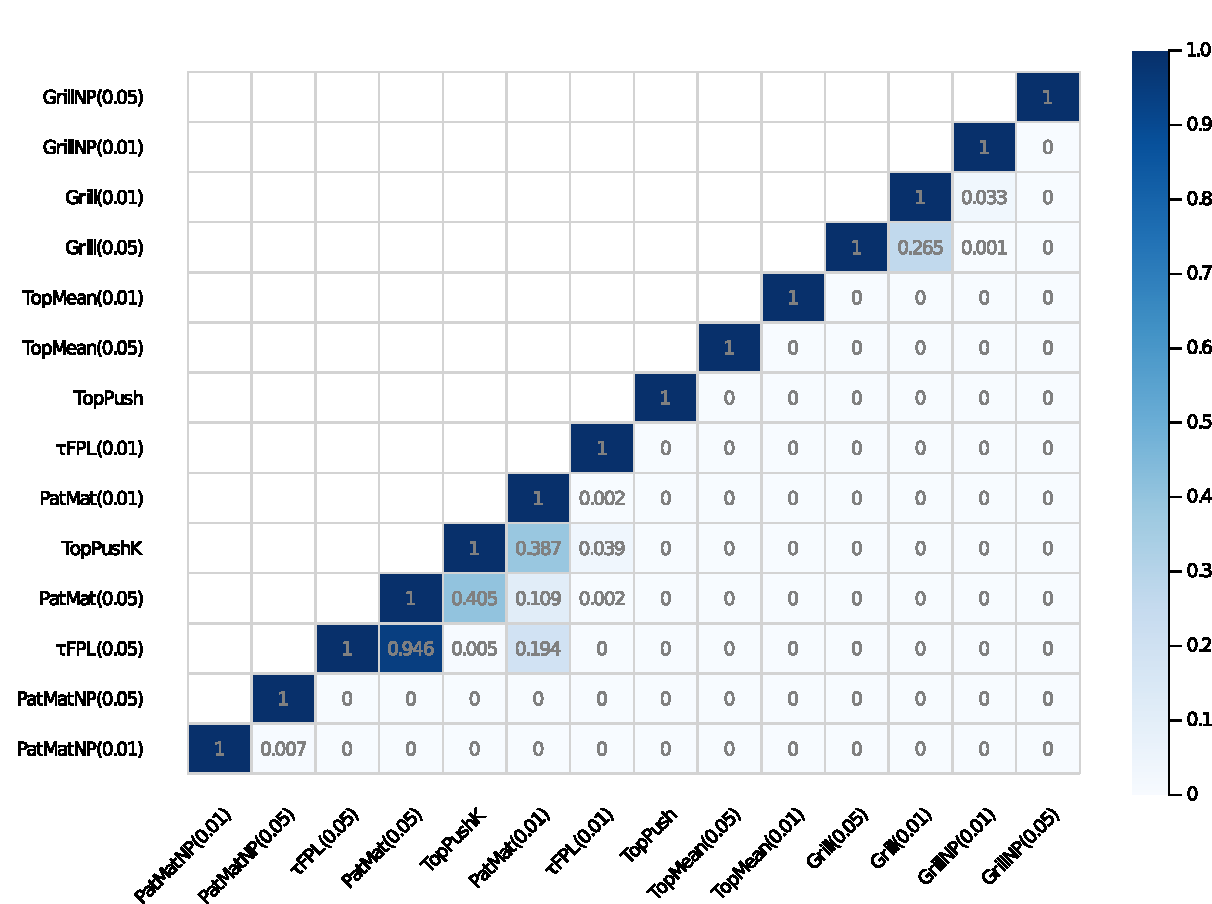
\includegraphics[width = \linewidth]{images/wilcoxon_fpr_1.pdf}
  \caption{The~$p$-value for the parwise Wilcoxon signed-rank test, where the null hypothesis is that the mean tpr@fpr(0.01) of both methods is the same. The methods are sorted by mean rank (left = better).}
  \label{fig:wilcoxon}
\end{figure}

Table~\ref{tab:fails} investigates the impact of~$\bm{w}=0$ as a potential global minimum. Each method was optimized for six different values of hyperparameters. The table depicts the condition under which the final value has a lower objective than~$\bm{w}=0$. Thus, \yesmark\ means that it is always better while \nomark\ means that the algorithm made no progress from the starting point~$\bm{w} =0$. The latter case implies that~$\bm{w}=0$ seems to be the global minimum. We make the following observations:
\begin{itemize}
  \item \PatMat and \PatMatNP are the only methods which succeeded at every dataset for some hyperparameter. Moreover, for each dataset, there was some~$\beta_0$ such that these methods were successful if and only if~$\beta\in(0,\beta_0)$. This is in agreement with Theorem~\ref{thm:patmat_zero}.
  \item \TopMeanK fails everywhere which agrees with Corollary~\ref{cor:topmean}.
  \item Figure~\ref{fig:thresholds} states that the methods from Section~\ref{sec: aatp} has a higher threshold than their Neyman-Pearson variants from Section~\ref{sec: Neyman-Pearson}. This is documented in the table as the latter have a higher number of successes.
\end{itemize}

\begin{table}[!ht]
  \centering
  \begin{tabular}{@{}lllll@{}}
    \toprule
    & Ionosphere & Hepmass & FashionMNIST & CIFAR100 \\
    \midrule
    \TopPush
      & \yesmark & \nomark & \yesmark & \nomark \\
    \TopPushK
      & \yesmark & \nomark & \yesmark & \nomark \\
    \Grill$\tau=0.01$
      & \nomark & \nomark & \nomark & \nomark \\
    \phantom{\Grill}$\tau=0.05$
      & \nomark &\nomark & \nomark & \nomark \\
    \PatMat$\tau=0.01$
      & \yesmark & \good{\boldmath$\beta\le 0.1$} & \good{\boldmath$\beta\le 1$} & \good{\boldmath$\beta\le 1$} \\
    \phantom{\PatMat}$\tau=0.05$
      & \yesmark & \good{\boldmath$\beta\le 1$} & \yesmark & \yesmark \\
    \TopMeanK$\tau=0.01$
      & \nomark & \nomark & \nomark & \nomark \\
    \phantom{\TopMeanK}$\tau=0.05$
      & \nomark & \nomark & \nomark & \nomark \\
    \GrillNP$\tau=0.01$
      & \nomark & \nomark & \nomark & \nomark \\
    \phantom{\GrillNP}$\tau=0.05$
      & \nomark & \nomark & \nomark & \nomark \\
    \PatMatNP$\tau=0.01$
      & \yesmark & \good{\boldmath$\beta\le 1$} & \yesmark & \good{\boldmath$\beta\le 1$} \\
    \phantom{\PatMatNP}$\tau=0.05$
      & \yesmark & \yesmark & \yesmark & \good{\boldmath$\beta\le 1$} \\
    \tauFPL$\tau=0.01$
      & \yesmark & \nomark & \yesmark & \nomark \\
    \phantom{\tauFPL}$\tau=0.05$
      & \yesmark & \yesmark & \yesmark & \good{\boldmath$\lambda\le 0.001$} \\
    \bottomrule
  \end{tabular}
  \caption{Necessary hyperparameter choice for the solution to have a better objective than zero. \yesmark\ means that the solution was better than zero for all hyperparameters while \nomark\ means that it was worse for all hyperparameters.}
  \label{tab:fails}
\end{table}

\section{Conclusion}

In this paper, we achieved the following results:
\begin{itemize}
  \item We presented a unified framework for the three criteria from Chapter~\ref{chap: framework}. These criteria include ranking, accuracy at the top and hypothesis testing.
  \item We showed that several known methods (\TopPush, \Grill, \tauFPL) fall into our framework and derived some completely new methods (\PatMat, \PatMatNP).
  \item We performed a theoretical analysis of the methods. We showed that known methods suffer from certain disadvantages. While \TopPush and \tauFPL are sensitive to outliers, \Grill is non-convex. We proved the global convergence of the stochastic gradient descent for \PatMat and \PatMatNP.
  \item We performed a numerical comparison and we showed a good performance of our method \PatMatNP.
\end{itemize}